\section{Lec 7}

\subsection{Equivalence Principle}

The idea of the \emph{universality} of the gravitational interaction, in the form of the \emph{Equivalence principle } led Einstein to think that gravity is one of a kind, not just another field, but a metric tensor that describes the curvature of spacetime.

\subsubsection{Weak Equivalence Principle, WEP}
It states that \emph{inertial} mass and \emph{gravitational} mass of any object are equal. \par
From the Second Law of Mechanics:
\[
 \vec{F}= m_{i}\vec{a}
\]
with $m_{i}=$ inertial mass.
While, to quantify gravitational forces in Newtonian mechanics:
\[
\vec{F} = -m_{g} \nabla \Phi_{g}
\]
With $\nabla \Phi_{g}$ gradient of scalar field $\Phi_{g}$, known as gravitational potential.
From these formulas, we see no actual reason why $m_{i} = m_{g}$:
\begin{itemize}
	\item The inertial mass has a universal character, it takes the same value no matter what kind of force is being exerted.
	\item The gravitational mass is a quantity specific to the gravitational force. One could think $ \frac{m_{g}}{m_{i}}$ as the \emph{gravitational charge}.
\end{itemize}
Galileo showed by rolling balls down the inclined plane that the response of matter to gravitation is universal, and in Newtonian mechanics it translates in WEP:
\[
m_{i }= m_{g}
\]
This, for freely falling objects, becomes
\[
a = -\nabla \Phi 
\]

This led to think an equivalent formulation of WEP that is: \emph{there exists a preferred class of trajectories through space time, called Inertial or Freely-Falling}.
Freely falling is intended as "moving under the sole influence of gravity", these objects are unaccelerated. \par

The universality of gravitation can be stated in another form:
\indent If we consider a physicist in a spaceship that is accelerating at a constant rate, like
\[
\vec{a} = - \vec{g}
\]
he would be not able to distinguish by scientific experiments the situation in which he sits on Earth's surface. (Restricted to local observation).


\tikzset{every picture/.style={line width=0.75pt}} %set default line width to 0.75pt

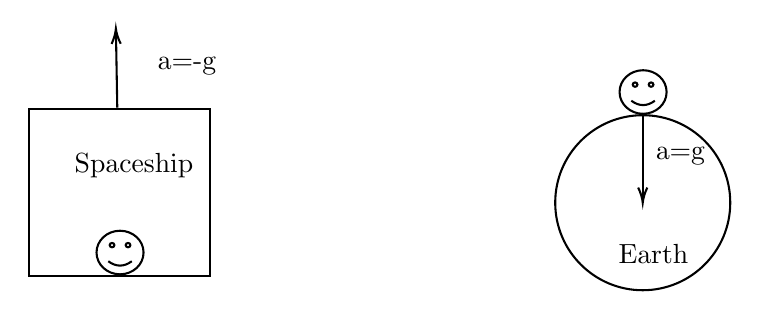
\begin{tikzpicture}[x=0.5pt,y=0.5pt,yscale=-1,xscale=1]
%uncomment if require: \path (0,300); %set diagram left start at 0, and has height of 300

%Shape: Rectangle [id:dp8176008658551641]
\draw   (98,85.5) -- (229,85.5) -- (229,206.5) -- (98,206.5) -- cycle ;
%Shape: Circle [id:dp5519338819044518]
\draw   (478.5,153.25) .. controls (478.5,118.32) and (506.82,90) .. (541.75,90) .. controls (576.68,90) and (605,118.32) .. (605,153.25) .. controls (605,188.18) and (576.68,216.5) .. (541.75,216.5) .. controls (506.82,216.5) and (478.5,188.18) .. (478.5,153.25) -- cycle ;
%Shape: Smiley Face [id:dp2317824195662611]
\draw   (147,189.25) .. controls (147,180.55) and (154.61,173.5) .. (164,173.5) .. controls (173.39,173.5) and (181,180.55) .. (181,189.25) .. controls (181,197.95) and (173.39,205) .. (164,205) .. controls (154.61,205) and (147,197.95) .. (147,189.25) -- cycle ; \draw   (156.52,183.9) .. controls (156.52,183.03) and (157.28,182.32) .. (158.22,182.32) .. controls (159.16,182.32) and (159.92,183.03) .. (159.92,183.9) .. controls (159.92,184.76) and (159.16,185.47) .. (158.22,185.47) .. controls (157.28,185.47) and (156.52,184.76) .. (156.52,183.9) -- cycle ; \draw   (168.08,183.9) .. controls (168.08,183.03) and (168.84,182.32) .. (169.78,182.32) .. controls (170.72,182.32) and (171.48,183.03) .. (171.48,183.9) .. controls (171.48,184.76) and (170.72,185.47) .. (169.78,185.47) .. controls (168.84,185.47) and (168.08,184.76) .. (168.08,183.9) -- cycle ; \draw   (155.5,195.55) .. controls (161.17,199.75) and (166.83,199.75) .. (172.5,195.55) ;
%Shape: Smiley Face [id:dp04372115955443423]
\draw   (525,73.25) .. controls (525,64.55) and (532.61,57.5) .. (542,57.5) .. controls (551.39,57.5) and (559,64.55) .. (559,73.25) .. controls (559,81.95) and (551.39,89) .. (542,89) .. controls (532.61,89) and (525,81.95) .. (525,73.25) -- cycle ; \draw   (534.52,67.9) .. controls (534.52,67.03) and (535.28,66.32) .. (536.22,66.32) .. controls (537.16,66.32) and (537.92,67.03) .. (537.92,67.9) .. controls (537.92,68.76) and (537.16,69.47) .. (536.22,69.47) .. controls (535.28,69.47) and (534.52,68.76) .. (534.52,67.9) -- cycle ; \draw   (546.08,67.9) .. controls (546.08,67.03) and (546.84,66.32) .. (547.78,66.32) .. controls (548.72,66.32) and (549.48,67.03) .. (549.48,67.9) .. controls (549.48,68.76) and (548.72,69.47) .. (547.78,69.47) .. controls (546.84,69.47) and (546.08,68.76) .. (546.08,67.9) -- cycle ; \draw   (533.5,79.55) .. controls (539.17,83.75) and (544.83,83.75) .. (550.5,79.55) ;
%Straight Lines [id:da28786648084951405]
\draw    (162,84.5) -- (161.04,29.5) ;
\draw [shift={(161,27.5)}, rotate = 88.99] [color={rgb, 255:red, 0; green, 0; blue, 0 }  ][line width=0.75]    (10.93,-3.29) .. controls (6.95,-1.4) and (3.31,-0.3) .. (0,0) .. controls (3.31,0.3) and (6.95,1.4) .. (10.93,3.29)   ;
%Straight Lines [id:da9125944015659164]
\draw    (541.75,90) -- (541.75,151.25) ;
\draw [shift={(541.75,153.25)}, rotate = 270] [color={rgb, 255:red, 0; green, 0; blue, 0 }  ][line width=0.75]    (10.93,-3.29) .. controls (6.95,-1.4) and (3.31,-0.3) .. (0,0) .. controls (3.31,0.3) and (6.95,1.4) .. (10.93,3.29)   ;

% Text Node
\draw (189,46) node [anchor=north west][inner sep=0.75pt]   [align=left] {a=-g};
% Text Node
\draw (549,111) node [anchor=north west][inner sep=0.75pt]   [align=left] {a=g};
% Text Node
\draw (522,181) node [anchor=north west][inner sep=0.75pt]   [align=left] {Earth};
% Text Node
\draw (129,115) node [anchor=north west][inner sep=0.75pt]   [align=left] {Spaceship};


\end{tikzpicture}
\bigskip\hfill

If the spaceship would be sufficiently big, we would see that the effect of acceleration would always be in the same direction, while on the surface or the Earth we would see that it points towards the center of the earth, so radial vs straight parallel lines.\par
So WEP could be stated as \emph{the motion of freely-falling particles are the same in a gravitational field and a uniformly accelerated frame, in small enough regions of spacetime}. In larger regions there would be inhomogenities, which will lead to tidal forces.

\subsubsection{Einstein's Equivalence Principle, EEP}
The Einstein Equivalence Principle is just a little generalization of the WEP:
\begin{quote}
In small enough regions of spacetime, the laws of physics reduce to those of special relativity: it is impossible to detect the existence of gravitational field by means of local experiments.
\end{quote}
Consider a hydrogen atom, a bound state of a proton and an electron. Its mass
is actually less than the sum of the masses of the proton and electron considered
individually, because there is a negative binding energy—you have to put energy
into the atom to separate the proton and electron. According to the WEP, the  gravitational mass of the hydrogen atom is therefore less than the sum of the masses of its constituents; the gravitational field couples to electromagnetism (which holds the atom together) in exactly the right way to make the gravitational mass come out right. This means that not only must gravity couple to rest mass universally, but also to all forms of energy and momentum—which is practically the claim of the EEP.

It is the EEP that implies that we should attribute the action of gravity the curvature of spacetime.

We know that there is a class of preferred frames: Inertial Frames (where laws of dynamics are true).
We introduce a new class of frames: Freely Falling Frames, where \emph{ unaccelerated particles move only due to gravity.} \par
Obviously these frames must be local frames, otherwise, due to inhomogenities on the gravitational field, particles initially at rest will begin to move with respect to such frame.
\begin{figure}[h]
\centering
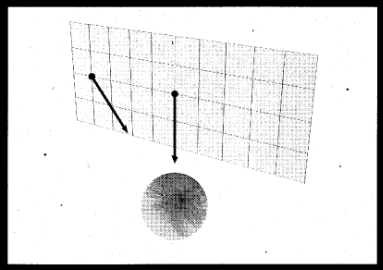
\includegraphics[width=0.8\linewidth]{imm/failureglobal.png}
\caption{The failure of global frames.}
\label{imm:failureglobal}
\end{figure}

After this we need a mathematical framework were what just said is consistent. The solution is to think that spacetime has a curved geometry and gravitation the manifestation of this curvature.
Before jumping in what is a manifold, let's see if the consequences are of our world.

\subsubsection{Gravitational Redshift}
\begin{figure}[h]
\centering
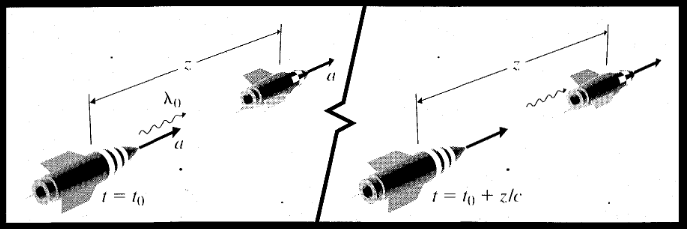
\includegraphics[width=0.8\linewidth]{imm/gravshift1.png}
\caption{Doppler shift measured by two rockets, each feeling acceleration \textbf{a}.}
\label{imm:gravshift1.png}
\end{figure}

Be two spaceships, separated by distance \emph{z}, each moving with constant $\vec{a}$ acceleration in a region without gravitational fields. \par
At \emph{t\textsubscript{0}} ship in the back emits a photos of $\lambda_{0}$.\par
The distance \emph{z} stays constant, so the photon is received after $\Delta t = z/c$ in our reference frame. At $t = t_{0}+ \Delta t$ spaceships have picked up an additional velocity $\Delta v = \vec{a}\Delta t = \vec{a}z/c$. The photon reaching the front spaceship will be redshifted by the Doppler Effect, by \[
\frac{\Delta \lambda }{\lambda_{0}} = \frac{\Delta v}{c} = \frac{a z}{c^{2}}
\]
And according to EEP this should happen also in a uniform gravitational field.\par
\begin{figure}[h]
\centering
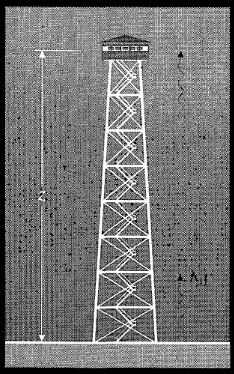
\includegraphics[width=0.3\linewidth]{imm/gravshift2.png}
\caption{Gravitational redshift on Earth's surface}
\label{imm:gravshift2}
\end{figure}
So if a photon is emitted from the ground with $\lambda_{0}$, it will be redshifted by
\[
\frac{\Delta  \lambda }{\lambda_{0}} = \frac{a_{g}z}{c^{2}}
\]
To note that is a direct consequence of EEP, no details of GR were required.
The thing is, if i try to represent this with Minkowski metric, I don't notice the redshift.

So now we really need to talk about Manifolds
\subsection{Manifolds}
A manifold is a space that may be curved and have a complicated topology, but in local regions looks just like $\mathbb{R}^{n}$. A crucial part is that the dimensionality \emph{n} of the Euclidean Spaces being used must be the same in every patch of the manifold.
For example are not manifolds, a line ending on a plane and two cones intersecting at their vertices.\par
\begin{figure}[h]
\centering
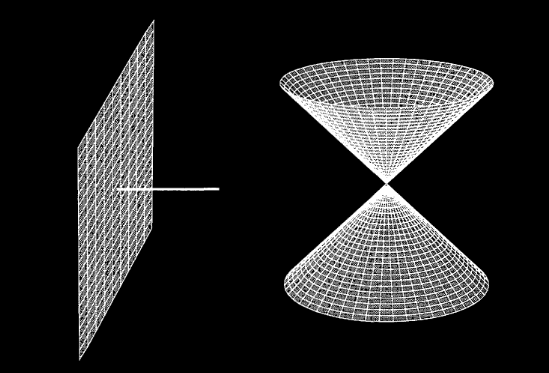
\includegraphics[width=0.5\linewidth]{imm/notmanifold.png}
\caption{Not manifolds}
\label{imm:notmanifold.png}
\end{figure}

\subsubsection{Coordinate System}
Be 
\begin{equation}
\begin{cases}
U\subset M \\
\phi : U \to \mathbb{R}^{n} \\
\phi\left( U \right) \text{ is open in }\mathbb{R}^{n}
\end{cases}
\end{equation}
These are a system of conditions to define a coordinate system or \emph{chart.}\par
\begin{figure}[h]
\centering
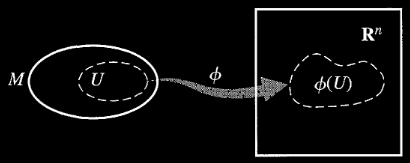
\includegraphics[width=0.65\linewidth]{imm/chart.png}
\caption{A coordinate chart covering an open subset \emph{U} of \emph{M}.}
\label{imm:chart}
\end{figure}
An \emph{atlas} is a indexed collection of charts $\{\left( U_{\alpha}, \phi_{\alpha } \right)\}$.

\subsubsection{Vectors again}
One point we stressed was the notion of a tangent space, the set of all vectors at a single point in spacetime. A vector is not a thing that stretches from one point to another but is an object associated with a single point. \par
Be $f : M \to \mathbb{R}$. Each curve passing through a point \emph{P}, defines an operator, the \emph{ directional derivative}, which maps $f \to df/d\lambda \left( \text{ at }p \right)$. \par
We claim the tangent space $T_{P}$ can be identified with the space of directional derivative operators along curves through \emph{P}.
And for any \emph{f} we can write:
\[
\frac{df}{d\lambda } = \frac{df}{dx^{\mu }} \frac{dx^{\mu }}{d\lambda } \implies \frac{d}{d\lambda } = \frac{dx^{\mu }}{d\lambda } \partial_{\mu }
\]
If i change the coordinates i can apply the chain rule.



\subsubsection{Strong Equivalence Principle, SEP}
I don't think during lectures we talked about this one. I'll post it here because I was curious.\par

Is defined to include all of the laws of physics, gravitational and otherwise.
We will define \emph{unaccelerated} as \emph{freely falling}, from here we decide that gravity is not a force, because a force leads to acceleration, and our definition of zero acceleration is \emph{ moving freely in the presence of whatever gravitational field happens to be around.} \par


